\documentclass[a4paper]{article}
\usepackage[utf8]{inputenc}
\usepackage[russian]{babel}
\usepackage[T2]{fontenc}
\usepackage[warn]{mathtext}
\usepackage{graphicx}
\usepackage{amsmath}
\usepackage{floatflt}
\usepackage[left=20mm, top=20mm, right=20mm, bottom=20mm, footskip=10mm]{geometry}


\graphicspath{ {images/} }
\usepackage{multicol}
\setlength{\columnsep}{2cm}


\begin{document}

\begin{titlepage}
	\centering
	\vspace{5cm}
	{\scshape\LARGE Московский физико-технический институт \par}
	\vspace{4cm}
	{\scshape\Large Лабораторная работа \par}
	\vspace{1cm}
	{\huge\bfseries Резонанс токов \par}
	\vspace{1cm}
	\vfill
\begin{flushright}
	{\large выполнили студенты 653 группы ФФКЭ}\par
	\vspace{0.3cm}
	{\LARGE Агафонов Владислав}
	
	
	{\LARGE Карпова Татьяна}
\end{flushright}
	

	\vfill

% Bottom of the page
	Долгопрудный, 2017 г.
\end{titlepage}

\section{Цель работы}

Исследование резонанса токов в параллельном колебательном контуре с изменяемой ёмкостью, включающее получение амплитудно-частотных и фазово-частотных характеристик, а также определение основных параметров контура.

\section{В работе используются:}
\begin{itemize}
    \item генератор сигналов
    \item источник тока, нагруженный на параллельный колебательный контур с переменной ёмкостью
    \item двулучевой осциллограф
    \item цифровые вольтметры
\end{itemize}


\section{Теоретические положения}

Схема экспериментального стенда для изучения резонанса токов в параллельном колебательном контуре показана на рис. 1. Синусоидальный сигнал от генератора GFG-8255A поступает на вход источника тока, собранного на операционном усилителе ОУ с полевым транзистором ПТ, питание которых осуществляется встроенным блоком-выпрямителем от сети переменного тока 220 вольт. Цепи питания на схеме не показаны, представлен только резистор, переменное напряжение, на котором в используемой схеме равно напряжению на входе «+» операционного усилителя. \\

\begin{figure}[h]
    \centering
    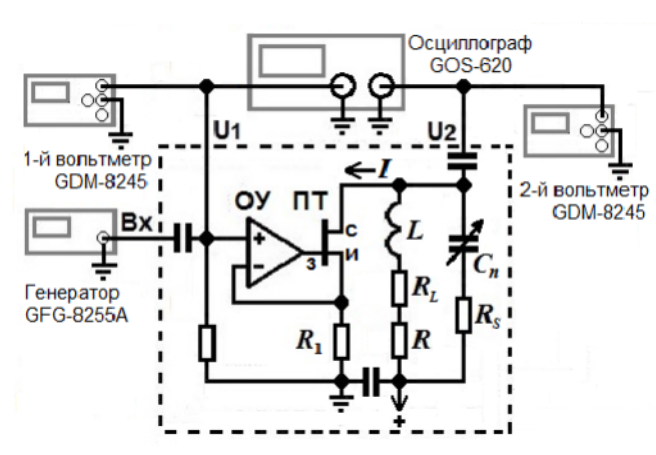
\includegraphics[width=10cm]{fig1.PNG}
    \caption{Схема экспериментального стенда}
    \label{fig:vac}
\end{figure}

Напряжение $ E = E_0cos(\omega t + \phi_0) $ поступает на вход «+» операционного усилителя от генератора через согласующую RC-цепочку. Это же напряжение через разъём «U1» подаётся одновременно на канал 1 осциллографа GOS-620 и вход 1-го цифрового вольтметра GDM-8245. Переменное напряжение на резисторе R1, как отмечалось выше, при этом также равно Е. Напряжение на контуре U, совпадающее с напряжением на конденсаторе, подаётся со знаком «–» через разъём «U2» на канал 2 осциллографа и вход 2-го цифрового вольтметра GDM-8245. Показанные на схеме установки ещё два конденсатора без наименований (помимо входящего в RC-цепочку) играют вспомогательную роль и не влияют на характеристики контура. Символ «->+» отмечает наличие источника питания полевого транзистора. Ток затвора «з» полевого транзистора ничтожно мал, так что токи истока «и» и стока «с» практически совпадают и равны току во внешней цепи контура. Как видно из схемы, \[ I = \frac{E}{R_1} = I_0cos(\omega t + \phi_0), \:\:\: I_0 = \frac{E_0}{R_1} \]


\section{Ход работы}
\begin{enumerate}
    \item Проведём измерения характеристик контура при разных значениях ёмкости конденсатора. Будем фиксировать резонансные частоты $f$ и напряжения $U$ в контуре при разных $C$, так же регистрируя входное напряжение $E$. Результаты измерений занесём в таблицу 1. При расчётах импеданса при резонансе $Z_r_e_s$, добротности контура $Q$, суммарного сопротивления $R_{\Sigma}$, реактивного сопротивления $\rho$, эквивалентного последовательного сопротивления конденсатора $R_s_m_a_x$ были использованы формулы:
    
\begin{center}
    $Z_r_e_s = \frac{U}{I_0} = \frac{U}{E/R_1}$ \hspace{1cm} $\rho = \sqrt{\frac{L}{C}}$\hspace{1cm} $Q = \frac{Z_r_e_s}{\rho}$ \\
    $R_{\Sigma} = \frac{Z_r_e_s}{Q^2}$ \hspace{1cm} $R_s_m_a_x = \frac{tg\delta}{\omega C}$ \hspace{1cm} $R_L = R_s_m_a_x - R$
    
\end{center}
    
    \begin{table}[h]
    \centering
    \begin{center}
    \caption{Измерения характеристик контура при разных ёмкостях}
    \end{center}
    \vspace{0.1cm}
    \label{tab:my_label}
    \begin{tabular}{ |p{1.2cm}|p{1.2cm}|p{0.9cm}|p{0.9cm}|p{1.3cm}|p{1.2cm}|p{1.5cm}|p{1.2cm}|p{1.2cm}|p{1.3cm}|p{1.2cm}| }
 \hline
$Cn,$ нФ & $f,$ кГц & $E,$ В & $U,$ В & $L,$ мкГн & $\rho,$ Ом & $Z_r_e_s,$ Ом & $Q$ & $R_{\Sigma}, $Ом & $R_m_a_x, $Ом & $R_L$, Ом\\
 \hline
25.100 & 32.113 & 0.350 & 2.056 & 978.599 & 197.454 & 5926.936 & 30.017 & 6.578 & 0.198 & 2.881\\
 \hline
33.200 & 27.886 & 0.349 & 1.582 & 981.137 & 171.908 & 4574.747 & 26.612 & 6.460 & 0.172 & 2.788\\
 \hline
47.300 & 23.186 & 0.349 & 1.155 & 996.156 & 145.122 & 3337.934 & 23.001 & 6.309 & 0.145 & 2.664\\
 \hline
57.400 & 21.248 & 0.349 & 0.986 & 977.445 & 130.494 & 2847.052 & 21.818 & 5.981 & 0.131 & 2.351\\
 \hline
67.500 & 19.472 & 0.349 & 0.835 & 989.727 & 121.089 & 2415.614 & 19.949 & 6.070 & 0.121 & 2.449\\
 \hline
82.700 & 17.700 & 0.349 & 0.706 & 977.661 & 108.728 & 2042.610 & 18.786 & 5.788 & 0.109 & 2.179\\
 \hline
101.600 & 16.070 & 0.348 & 0.587 & 965.417 & 97.479 & 1697.456 & 17.414 & 5.598 & 0.098 & 2.000\\
\hline
\hline
    

    \end{tabular}
\end{table}

Рассчитаем погрешности определения индуктивности катушки и сопротивления катушки.

\begin{center}
    $L_a_v = 980.877$ мкГн \hspace{1cm} $R_L_a_v = 2.473$ Ом \hspace{1cm} среднее значение\\
    $L_{dev.eq} = 3.710 $мкГн \hspace{1cm} $R_L_{dev.eq} = 0.122$ Ом\hspace{1cm} среднеквадратичное отклонение\\
    $\sigma_L = 9.079 $мкГн \hspace{1cm} $\sigma_R = 0.299$ Ом\hspace{1cm} случайная погрешность \\ 
\end{center}


    \item Снимем амплитудно-частотную характеристику контура при ёмкостях $C_2$ и $C_4$. Для этого будем снимать зависимость напряжения в контуре от частоты колебаний. Результаты измерений занесём в табл. 2, резонансные кривые $U(f)$ представим на рис. 2
    
\begin{table}[h]
    \centering
    \begin{center}
    \caption{Зависимость частоты колебаний от напряжения}
    \end{center}
    \vspace{0.1cm}
    \label{tab:my_label}
    \begin{tabular}{ |p{2cm}|p{2cm}||p{2cm}|p{2cm}|}
 \hline
 \multicolumn{2}{|c|}{$C_2$} & \multicolumn{2}{c|}{$C_4$} \\
 \hline
    $f, $Гц & $U, $В &  $f, $Гц & $U, $В \\
\hline
    17.012 & 0.0581	& 12.740 &	0.0424 \\
    \hline
17.861 &	0.0648 &	13.190 &	0.0458 \\
    \hline
18.687 &	0.0725 &	14.092 &	0.0536 \\
    \hline
19.034 &	0.0762 &	14.918 &	0.0625 \\
    \hline
20.257 &	0.0916 &	15.513 &	0.0704 \\
    \hline
21.401 &	0.1110 &	16.366 &	0.0851 \\
    \hline
22.510 &	0.1376 &	17.847 &	0.1270 \\
    \hline
23.827 &	0.1878 &	18.160 &	0.1407 \\
    \hline
24.810 &	0.2524 &	19.155 &	0.2093 \\
    \hline
25.430 &	0.3146 &	19.858 &	0.3094 \\
    \hline
25.786 &	0.3739 &	20.342 &	0.4496 \\
    \hline
26.176 &	0.4578 &	20.833 &	0.7330 \\
    \hline
26.964 &	0.8016 &	21.140 &	0.9554 \\
    \hline
27.394 &	1.2200 &	21.233 &	0.9846 \\
    \hline
27.627 &	1.4952 &	21.539 &	0.8210 \\
    \hline
27.931 &	1.5576 &	21.884 &	0.6205 \\
    \hline
28.373 &	1.0974 &	22.285 &	0.4339 \\
    \hline
29.188 &	0.5811 &	23.074 &	0.2673 \\
    \hline
30.062 &	0.3737 &	24.022 &	0.1821 \\
    \hline
31.011 &	0.2690 &	24.771 &	0.1460 \\
    \hline
32.190 &	0.2008 &	25.222 &	0.1306 \\
    \hline
34.125 &	0.1433 &	26.031 &	0.1103 \\
    \hline
34.816 &	0.1305 &	27.071 &	0.0924 \\
    \hline
35.326 &	0.1226 &	27.880 &	0.0823 \\
    \hline
36.193 &	0.1111 &	28.500 &	0.0760 \\
    \hline
37.183 &	0.1009 &	29.031 &	0.0716 \\
    \hline
38.216 &	0.0920 &	29.647 &	0.0670 \\
    \hline
39.663 &	0.0823 & & \\	
    \hline
    \end{tabular}
\end{table} 



\begin{figure}[h]
    \centering
    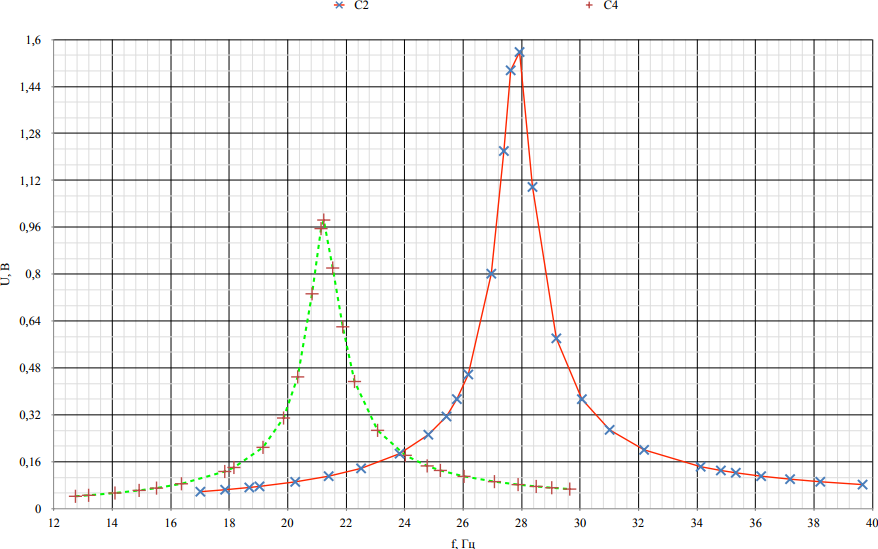
\includegraphics[width=\textwidth]{graph1.PNG}
    \caption{АЧХ контуров с С2 и С4}
    \label{fig:vac}
\end{figure}

Проведём сравнительный анализ АЧХ для двух ёмкостей в контуре. $C_4 > C_2$, формула для добротности $Q = \frac{1}{R}\sqrt{\frac{L}{C}}$. При повышении ёмкости падает добротность контура.

    \item Построим графики АЧХ в координатах $U/U_0(f/f_0)$. По этим графикам (ширина резонансной кривой на уровне $\frac{1}{\sqrt{2}}$) определим добротность контуров.
    \begin{center}
        $Q = \frac{1}{\Pi_{0.7}}$ \\
        $Q_2 = 26.31$ \hspace{1cm} $Q_4 = 22.22$
    \end{center}
    
    Значения, определённые в пункте 1:
    
    \begin{center}
    $Q_2 = 26.62$ \hspace{1cm} $Q_4 = 21.82$    
    \end{center}
    
    Эти значения практически совпадают.
    
\begin{figure}[h]
    \centering
    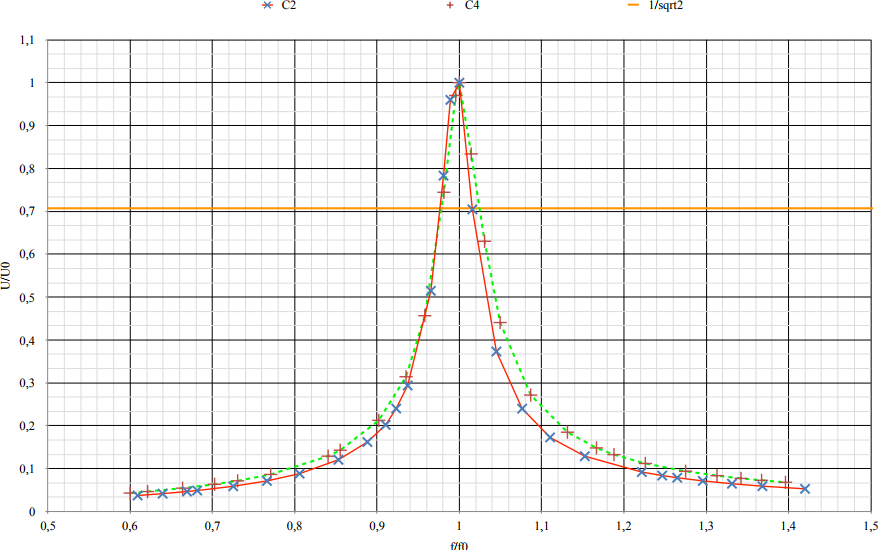
\includegraphics[width=\textwidth]{graph2.PNG}
    \caption{АЧХ контуров с С2 и С4 в относительных координатах}
    \label{fig:vac}
\end{figure}


    \item Построим ФЧХ для контура с $C_2$ в координатах $x = f/f_0 \;\;\; y = \varphi/\pi   $ (рис. 5). По графику определим добротность контура следующим методом: расстояние между точками по оси $x$, в которых $y$ меняется от $-\pi/4$ до $\pi/4$, равно $1/Q$. 
    
    $$Q = \frac{1}{1,002-0,966} \approx 27,7$$
    
    
    \begin{figure}[h]
    \centering
    \includegraphics[width=\textwidth]{tab.png}
    \caption{ФЧХ контура $C_2$, результаты измерений}
    \label{fig:vac}
\end{figure}
    
    \begin{figure}[h]
    \centering
    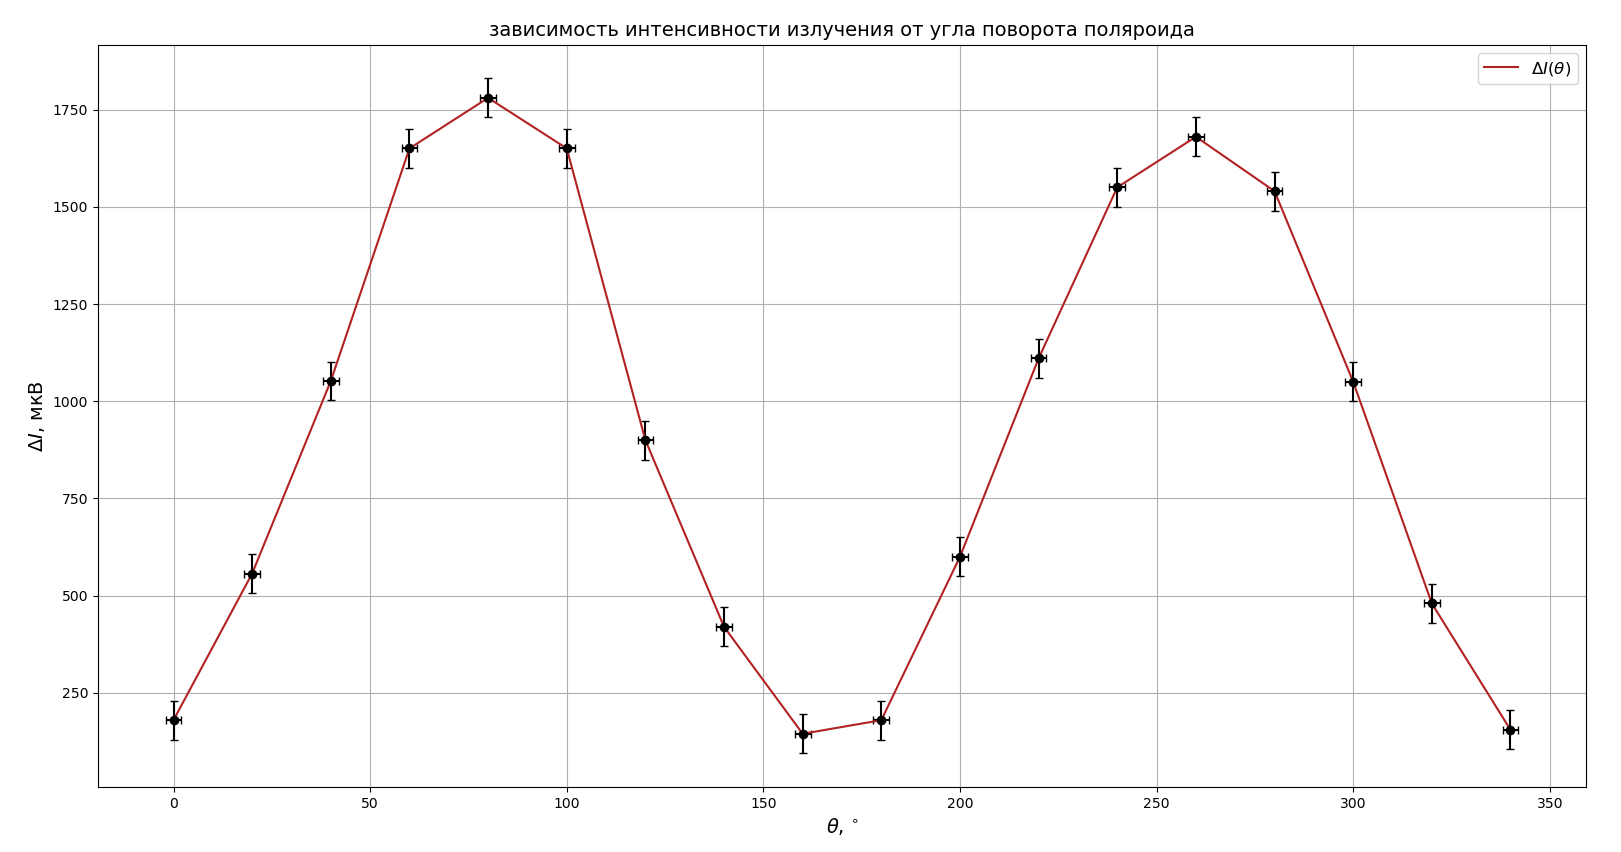
\includegraphics[width=\textwidth]{graph.png}
    \caption{ФЧХ контура $C_2$}
    \label{fig:vac}
\end{figure}

\newpage

\item Построим векторную диаграмму для токов и напряжений в контуре. Определим значения токов на конденсаторе и на катушке, а также напряжение в контуре,  резонансе по формулам
\begin{center}
    $I_0 = \frac{E}{R_1} = 0.0034 A$ $I_c = I_L = Q I_0 = \frac{Q E}{R_1} = 0.006 A$ \hspace{1cm} $U = Q\rho I_0 = \frac{Q\rhp E}{R_1} = 0.586 B$
\end{center}
    
    Также определим сдвиги по фазе их от основного тока $I_0$:
    \begin{center}
        $\varphi_c = \frac{\pi}{4} - \frac{R + R_L}{\rho} = 86.7 ^{\circ}$ \hspace{1cm} $\varphi_L = -\frac{\pi}{2} + \delta = 90 ^{\circ}$ \hspace{1cm} $\varphi_U = \frac{R + R_L}{\rho} + \delta = 3.2 ^{\circ} $
    \end{center}
    
    \begin{figure}[h]
    \centering
    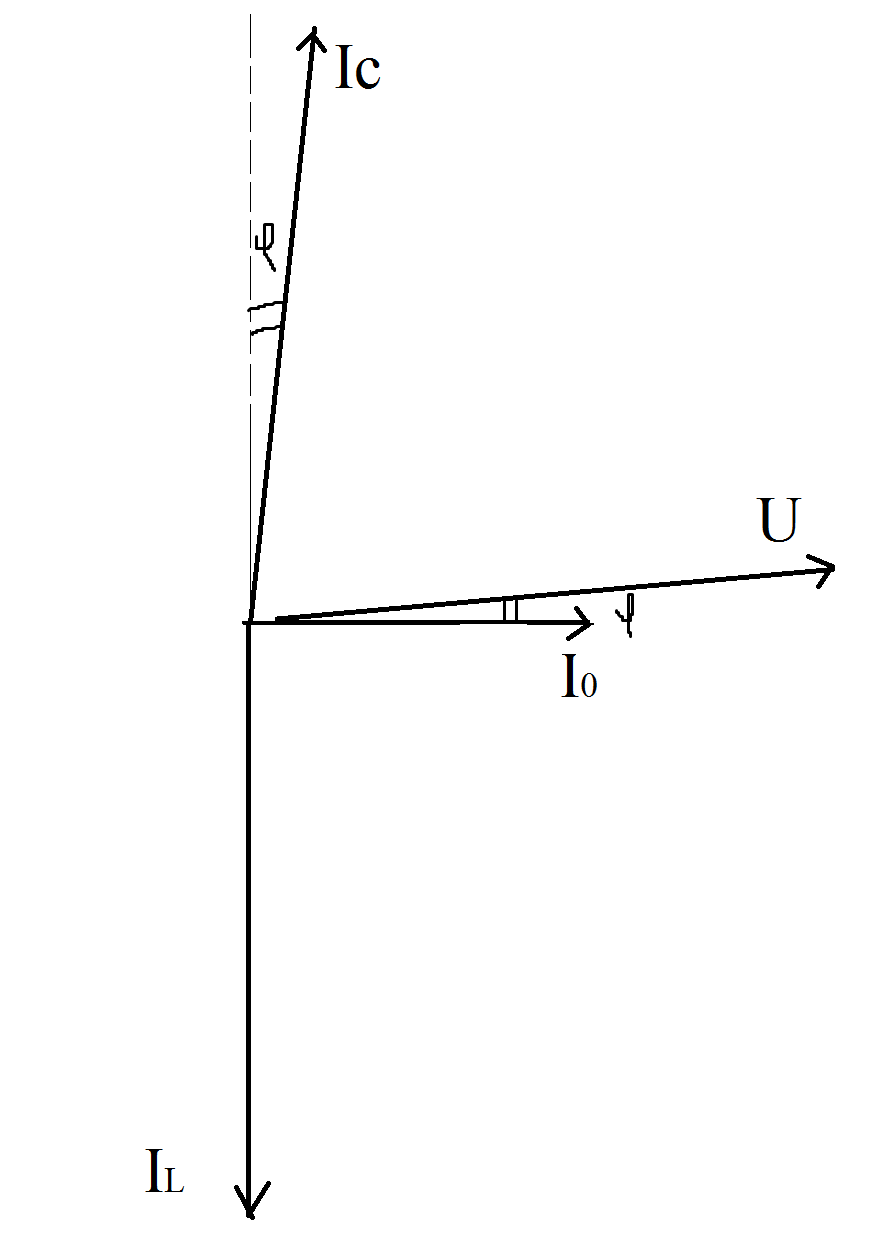
\includegraphics[width=10cm]{graph4.png}
    \caption{Векторная диаграмма токов и напряжения для контура с добротностью $Q = 17.414$}
    \label{fig:vac}
\end{figure}
    
\end{enumerate}

\section{Вывод}
В ходе работы мы ознакомились с явлением резонанса токов, изучили метод комплексных амплитуд, изучили амплитудно-частотные и фазово-частотную характеристику колебательного контура, составленного из элементов, используемых в современной радиотехнике. В ходе эксперимента была с большой точностью разными методами определена добротность колебательного контура при разных значениях ёмкости конденсатора в цепи, а также рассчитаны некоторые другие характеристики контура. Результаты определения добротности непосредственными измерениями параметров контура, методом резонансных кривых и по исследованию ФЧХ совпадают. \par
Также было исследовано само поведение токов и напряжений в контуре. Выяснено, какой вклад вносят в цепь сопротивление конденсатора (очень незначительный) и катушки (порядка сопротивления резистора в цепи). Численно получено значение индуктивности катушки и её сопротивления. Сделан вывод, что при точном расчёте цепей обязательно нужно учитывать сопротивление катушки. Была также построена векторная диаграмма токов и напряжений в исследуемом контуре, изучена природа явления резонанса токов.

\end{document}
